\documentclass[border=5pt]{standalone}
\usepackage{tikz}

\begin{document}

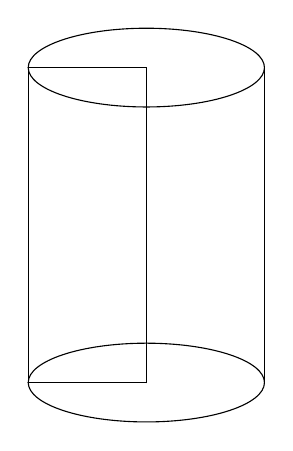
\begin{tikzpicture}[line cap=round, line join=round, >=stealth]
    % Variables for easy adjustment
    \def\r{1.5}  % radius
    \def\h{4}    % height

    % Draw the top ellipse
    \draw (0,\h) ellipse (\r cm and 0.5cm);

    % Draw the bottom visible curve
    \draw (-\r,0) arc (180:360:\r cm and 0.5cm);

    \draw (-\r,0) arc (180:0:\r cm and 0.5cm);

    % Draw vertical side lines
    \draw (-\r,0) -- (-\r,\h);
    \draw (\r,0) -- (\r,\h);

    % Draw the internal cross-section (the "L" shape from the image)
    % Center axis
    \draw (0,0) -- (0,\h);

    % Radius lines (top and bottom)
    \draw (0,\h) -- (-\r,\h);
    \draw (0,0) -- (-\r,0);

\end{tikzpicture}

\end{document}
